% Options for packages loaded elsewhere
\PassOptionsToPackage{unicode}{hyperref}
\PassOptionsToPackage{hyphens}{url}
\PassOptionsToPackage{dvipsnames,svgnames,x11names}{xcolor}
%
\documentclass[
  ignorenonframetext,
]{beamer}
\usepackage{pgfpages}
\setbeamertemplate{caption}[numbered]
\setbeamertemplate{caption label separator}{: }
\setbeamercolor{caption name}{fg=normal text.fg}
\beamertemplatenavigationsymbolsempty
% Prevent slide breaks in the middle of a paragraph
\widowpenalties 1 10000
\raggedbottom

\usepackage{amsmath,amssymb}
\usepackage{iftex}
\ifPDFTeX
  \usepackage[T1]{fontenc}
  \usepackage[utf8]{inputenc}
  \usepackage{textcomp} % provide euro and other symbols
\else % if luatex or xetex
  \usepackage{unicode-math}
  \defaultfontfeatures{Scale=MatchLowercase}
  \defaultfontfeatures[\rmfamily]{Ligatures=TeX,Scale=1}
\fi
\usepackage{lmodern}
\usetheme[]{AnnArbor}
\usecolortheme{dolphin}
\usefonttheme{structurebold}
\ifPDFTeX\else  
    % xetex/luatex font selection
\fi
% Use upquote if available, for straight quotes in verbatim environments
\IfFileExists{upquote.sty}{\usepackage{upquote}}{}
\IfFileExists{microtype.sty}{% use microtype if available
  \usepackage[]{microtype}
  \UseMicrotypeSet[protrusion]{basicmath} % disable protrusion for tt fonts
}{}
\makeatletter
\@ifundefined{KOMAClassName}{% if non-KOMA class
  \IfFileExists{parskip.sty}{%
    \usepackage{parskip}
  }{% else
    \setlength{\parindent}{0pt}
    \setlength{\parskip}{6pt plus 2pt minus 1pt}}
}{% if KOMA class
  \KOMAoptions{parskip=half}}
\makeatother
\usepackage{xcolor}
\newif\ifbibliography
\setlength{\emergencystretch}{3em} % prevent overfull lines
\setcounter{secnumdepth}{-\maxdimen} % remove section numbering


\providecommand{\tightlist}{%
  \setlength{\itemsep}{0pt}\setlength{\parskip}{0pt}}\usepackage{longtable,booktabs,array}
\usepackage{calc} % for calculating minipage widths
\usepackage{caption}
% Make caption package work with longtable
\makeatletter
\def\fnum@table{\tablename~\thetable}
\makeatother
\usepackage{graphicx}
\makeatletter
\def\maxwidth{\ifdim\Gin@nat@width>\linewidth\linewidth\else\Gin@nat@width\fi}
\def\maxheight{\ifdim\Gin@nat@height>\textheight\textheight\else\Gin@nat@height\fi}
\makeatother
% Scale images if necessary, so that they will not overflow the page
% margins by default, and it is still possible to overwrite the defaults
% using explicit options in \includegraphics[width, height, ...]{}
\setkeys{Gin}{width=\maxwidth,height=\maxheight,keepaspectratio}
% Set default figure placement to htbp
\makeatletter
\def\fps@figure{htbp}
\makeatother
% definitions for citeproc citations
\NewDocumentCommand\citeproctext{}{}
\NewDocumentCommand\citeproc{mm}{%
  \begingroup\def\citeproctext{#2}\cite{#1}\endgroup}
\makeatletter
 % allow citations to break across lines
 \let\@cite@ofmt\@firstofone
 % avoid brackets around text for \cite:
 \def\@biblabel#1{}
 \def\@cite#1#2{{#1\if@tempswa , #2\fi}}
\makeatother
\newlength{\cslhangindent}
\setlength{\cslhangindent}{1.5em}
\newlength{\csllabelwidth}
\setlength{\csllabelwidth}{3em}
\newenvironment{CSLReferences}[2] % #1 hanging-indent, #2 entry-spacing
 {\begin{list}{}{%
  \setlength{\itemindent}{0pt}
  \setlength{\leftmargin}{0pt}
  \setlength{\parsep}{0pt}
  % turn on hanging indent if param 1 is 1
  \ifodd #1
   \setlength{\leftmargin}{\cslhangindent}
   \setlength{\itemindent}{-1\cslhangindent}
  \fi
  % set entry spacing
  \setlength{\itemsep}{#2\baselineskip}}}
 {\end{list}}
\usepackage{calc}
\newcommand{\CSLBlock}[1]{\hfill\break\parbox[t]{\linewidth}{\strut\ignorespaces#1\strut}}
\newcommand{\CSLLeftMargin}[1]{\parbox[t]{\csllabelwidth}{\strut#1\strut}}
\newcommand{\CSLRightInline}[1]{\parbox[t]{\linewidth - \csllabelwidth}{\strut#1\strut}}
\newcommand{\CSLIndent}[1]{\hspace{\cslhangindent}#1}


% logo
\titlegraphic{
\includegraphics[width=4cm]{000_logos/logo-blue-vertical}}
\logo{\ifnum\thepage>1
\includegraphics[width=0.5cm]{000_logos/logo-blue-vertical}\fi}

% UMNG: Manual de image institucional

% Colors

% Umng
\definecolor{yellow}{HTML}{fdc600}
\definecolor{red}{HTML}{ee2a24}

% Estudios a Distancia
\definecolor{blue1}{HTML}{12245b}
\definecolor{blue2}{HTML}{767ca6}
\definecolor{blue3}{HTML}{cad2ec}

% Modify items
\setbeamercolor{palette primary}{bg=blue3}
\setbeamercolor{palette tertiary}{bg=blue1}
\setbeamercolor{frametitle}{bg=yellow}

% Hyperlinks
\hypersetup{
  linkcolor=red,
  citecolor=red
}

\makeatletter
\@ifpackageloaded{caption}{}{\usepackage{caption}}
\AtBeginDocument{%
\ifdefined\contentsname
  \renewcommand*\contentsname{Table of contents}
\else
  \newcommand\contentsname{Table of contents}
\fi
\ifdefined\listfigurename
  \renewcommand*\listfigurename{List of Figures}
\else
  \newcommand\listfigurename{List of Figures}
\fi
\ifdefined\listtablename
  \renewcommand*\listtablename{List of Tables}
\else
  \newcommand\listtablename{List of Tables}
\fi
\ifdefined\figurename
  \renewcommand*\figurename{Figure}
\else
  \newcommand\figurename{Figure}
\fi
\ifdefined\tablename
  \renewcommand*\tablename{Table}
\else
  \newcommand\tablename{Table}
\fi
}
\@ifpackageloaded{float}{}{\usepackage{float}}
\floatstyle{ruled}
\@ifundefined{c@chapter}{\newfloat{codelisting}{h}{lop}}{\newfloat{codelisting}{h}{lop}[chapter]}
\floatname{codelisting}{Listing}
\newcommand*\listoflistings{\listof{codelisting}{List of Listings}}
\makeatother
\makeatletter
\makeatother
\makeatletter
\@ifpackageloaded{caption}{}{\usepackage{caption}}
\@ifpackageloaded{subcaption}{}{\usepackage{subcaption}}
\makeatother

\ifLuaTeX
\usepackage[bidi=basic]{babel}
\else
\usepackage[bidi=default]{babel}
\fi
\babelprovide[main,import]{english}
% get rid of language-specific shorthands (see #6817):
\let\LanguageShortHands\languageshorthands
\def\languageshorthands#1{}
\ifLuaTeX
  \usepackage{selnolig}  % disable illegal ligatures
\fi
\usepackage{bookmark}

\IfFileExists{xurl.sty}{\usepackage{xurl}}{} % add URL line breaks if available
\urlstyle{same} % disable monospaced font for URLs
\hypersetup{
  pdftitle={Perception, Cognition, and Emotion},
  pdfauthor={Luis Francisco Gómez López},
  pdflang={en},
  colorlinks=true,
  linkcolor={Maroon},
  filecolor={Maroon},
  citecolor={Blue},
  urlcolor={Blue},
  pdfcreator={LaTeX via pandoc}}


\title{Perception, Cognition, and Emotion}
\author{Luis Francisco Gómez López}
\date{2024-07-26}
\institute{FAEDIS}

\begin{document}
\frame{\titlepage}

\renewcommand*\contentsname{Table of contents}
\begin{frame}[allowframebreaks]
  \frametitle{Table of contents}
  \tableofcontents[hideallsubsections]
\end{frame}

\section{Please Read Me}\label{please-read-me}

\begin{frame}{}
\phantomsection\label{section}
\begin{itemize}
\item
  Check the message \textbf{Welcome greeting} published in the News
  Bulletin Board.
\item
  Dear student please edit your profile uploading a photo where your
  face is clearly visible.
\item
  The purpose of the virtual meetings is to answer questions and not to
  make a summary of the study material.
\item
  This presentation is based on
  (\citeproc{ref-lewicki_negociacion_2024}{Lewicki, Barry, and Saunders
  2024, chap. 6})
\end{itemize}
\end{frame}

\section{Purpose}\label{purpose}

\begin{frame}{}
\phantomsection\label{section-1}
Understand how perceptions, knowledge and emotions affect a negotiation
process.
\end{frame}

\begin{frame}{}
\phantomsection\label{section-2}
\begin{itemize}
\item
  \textbf{Perception} is defined as the process by which individuals
  acquire information from their environment through the senses.

  \begin{itemize}
  \tightlist
  \item
    Individuals actively construct impressions based on this
    information, guiding their subsequent behavior
  \end{itemize}
\item
  The distortions of the perception may occur when the impressions that
  are generated don't reflect the real aspects of a situation.

  \begin{itemize}
  \tightlist
  \item
    This type of distortions are known as \textbf{cognitive biases}
  \end{itemize}
\end{itemize}
\end{frame}

\begin{frame}{}
\phantomsection\label{section-3}
\begin{itemize}
\tightlist
\item
  Example of a distortion in perception
\end{itemize}

\begin{figure}

\centering{

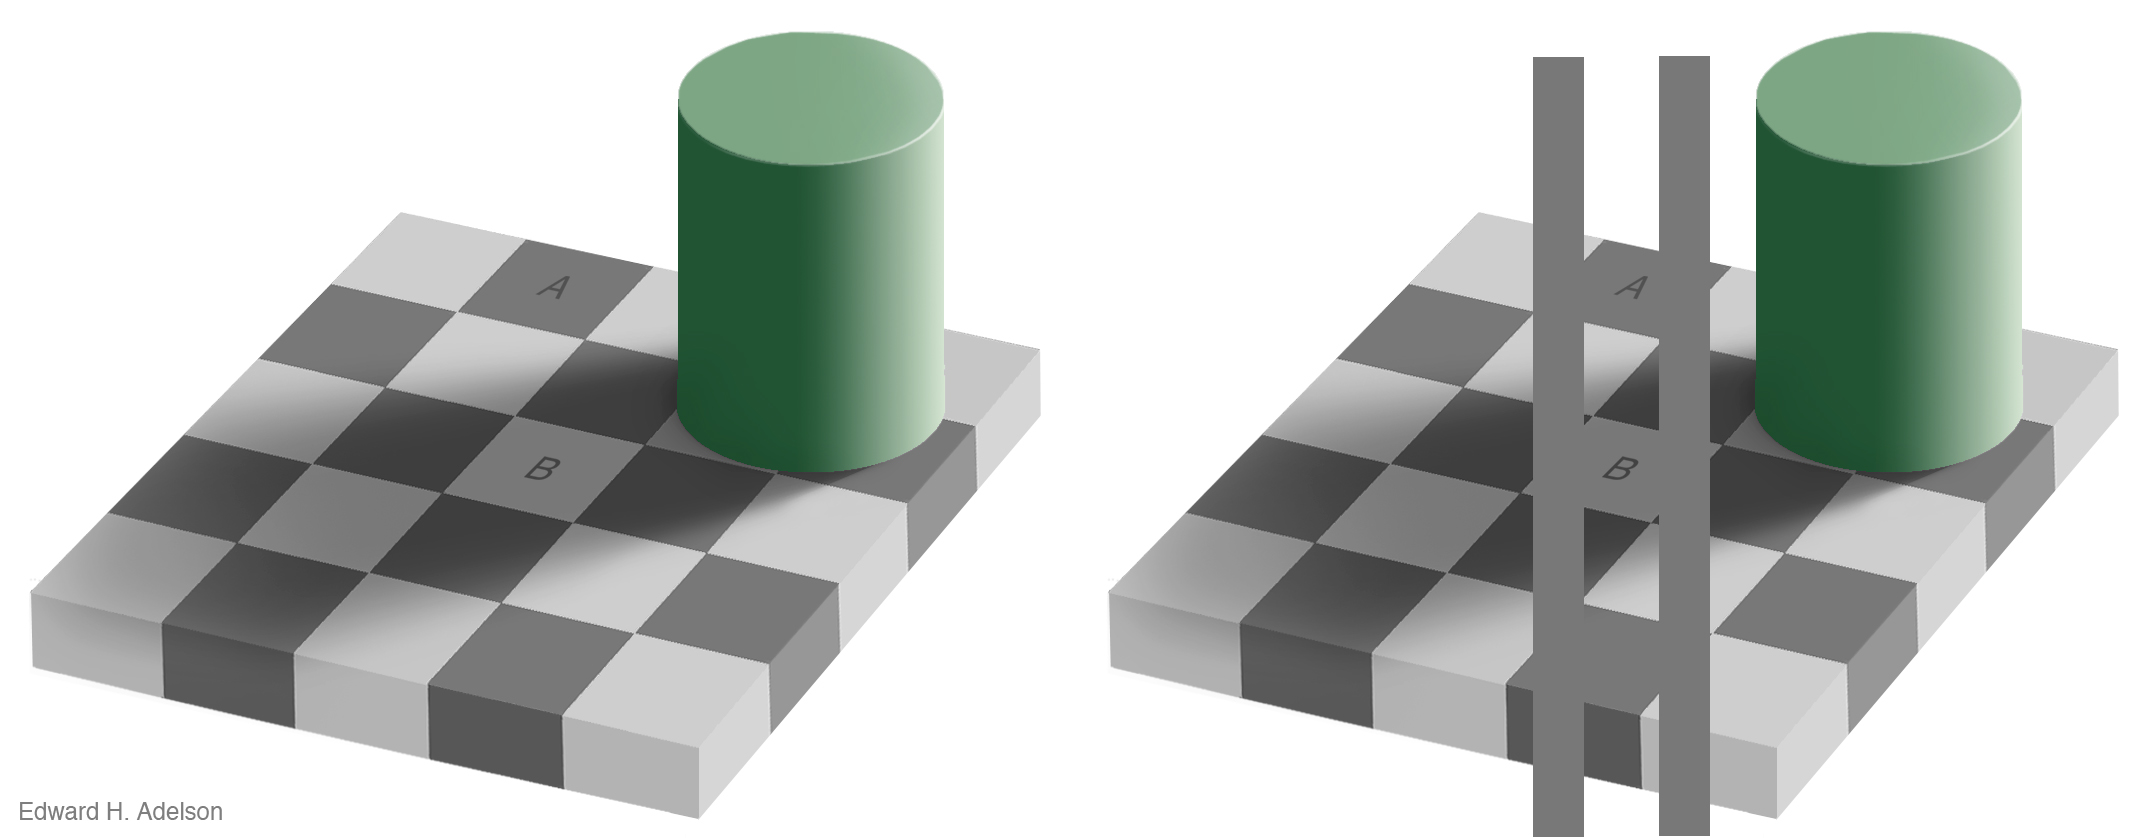
\includegraphics[width=4.16667in,height=4.16667in]{005_checkershadow_double_full.jpg}

}

\caption{\label{fig-checker-shadow-illusion}Checker Shadow illusion
(\citeproc{ref-adelson_checkershadow_1995}{Adelson 1995})}

\end{figure}%
\end{frame}

\begin{frame}{}
\phantomsection\label{section-4}
\begin{itemize}
\tightlist
\item
  Example of a distortion in perception
\end{itemize}

\begin{figure}

\centering{

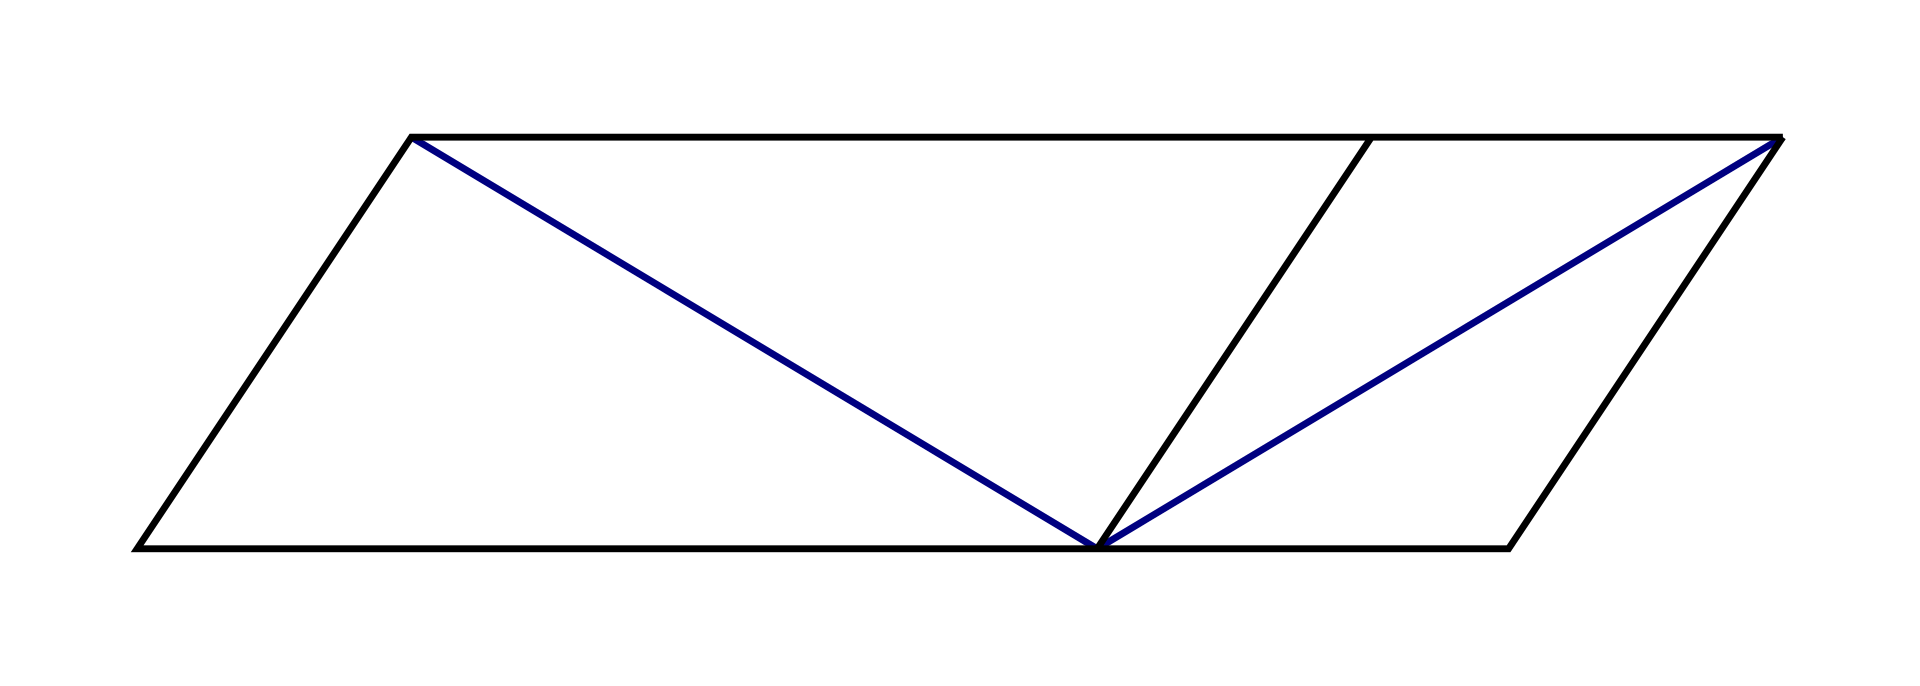
\includegraphics[width=4.16667in,height=4.16667in]{005_sander_Illusion.png}

}

\caption{\label{fig-sanders-parallelogram}Sander's parallelogram
(\citeproc{ref-luckiesh_visual_2017}{Luckiesh 2017})}

\end{figure}%
\end{frame}

\begin{frame}{}
\phantomsection\label{section-5}
\begin{itemize}
\tightlist
\item
  Example of a distortion in perception
\end{itemize}

\begin{figure}

\centering{

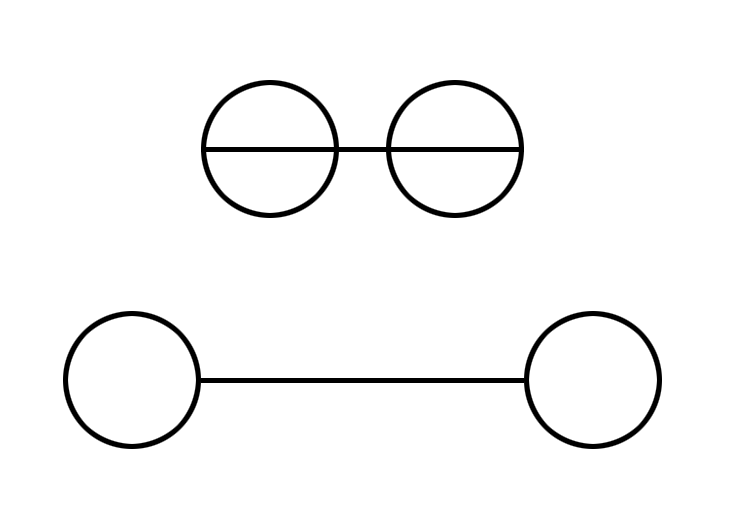
\includegraphics[width=3.125in,height=3.125in]{005_muller_lLyer_circle.png}

}

\caption{\label{fig-muller-lyer-illusion}Müller-Lyer Illusion
(\citeproc{ref-zeman_muller-lyer_2013}{Zeman et al. 2013})}

\end{figure}%
\end{frame}

\section{Framing}\label{framing}

\begin{frame}{}
\phantomsection\label{section-6}
\begin{itemize}
\item
  \textbf{Framing} is a concept initially coined by
  (\citeproc{ref-bateson_steps_2000}{Bateson 2000}) and developed by
  (\citeproc{ref-goffman_frame_1986}{Goffman 1986}).

  \begin{itemize}
  \tightlist
  \item
    It is defined as the interpretation schemes that individuals use to
    understand reality and act based on the interpretation they perform.
  \end{itemize}
\item
  In general terms, this means that individuals have built mental
  filters throughout their lives that allow them to understand the
  world. In turn, these mental filters influence the decisions they
  make.
\end{itemize}
\end{frame}

\begin{frame}{}
\phantomsection\label{section-7}
\begin{itemize}
\item
  Example of how \textbf{framing} can change decisions depending on how
  information is presented (\citeproc{ref-tversky_framing_1981}{Tversky
  and Kahneman 1981}, p 453):

  \begin{itemize}
  \item
    \textbf{Problem 1} {[}N = 152{]}\footnote<.->{Number of people that
      participate in the experiment}: Imagine that the U.S. is preparing
    for the outbreak of an unusual Asian disease, which is expected to
    kill 600 people. Two alternative programs to combat the disease have
    been proposed. Assume that the exact scientific estimate of the
    consequences of the programs are as follows:

    \begin{itemize}
    \tightlist
    \item
      If Program A is adopted, 200 people will be saved. \textbf{{[}72
      percent{]}}\footnote<.->{Percentage of people that choose Program
        A}
    \item
      If Program B is adopted, there is 1/3 probability that 600 people
      will be saved, and 2/3 probability that no people will be saved.
      \textbf{{[}28 percent{]}}\footnote<.->{Percentage of people that
        choose Program B}
    \end{itemize}
  \item
    Which of the two programs would you favor?
  \end{itemize}
\end{itemize}
\end{frame}

\begin{frame}{}
\phantomsection\label{section-8}
\begin{itemize}
\item
  Example of how \textbf{framing} can change decisions depending on how
  information is presented (\citeproc{ref-tversky_framing_1981}{Tversky
  and Kahneman 1981}, p 453):

  \begin{itemize}
  \item
    \textbf{Problem 2} {[}N = 155{]}\footnote<.->{Number of people that
      participate in the experiment}: The same statement as
    \textbf{Problem 1}

    \begin{itemize}
    \tightlist
    \item
      If Program C is adopted, 400 people will die. \textbf{{[}22
      percent{]}}\footnote<.->{Percentage of people that choose Program
        C}
    \item
      If Program D is adopted there is 1/3 probability that nobody will
      die, and 2/3 probability that 600 people will die. \textbf{{[}78
      percent{]}}\footnote<.->{Percentage of people that choose Program
        D}
    \end{itemize}
  \item
    Which of the two programs would you favor?
  \end{itemize}
\item
  \textbf{Problem 1} and \textbf{Problem 2} are equivalent but they are
  frame in a different way. This is why the majority choice in
  \textbf{Problem 1} is Program A and for the \textbf{Problem 2} is
  Program D.
\end{itemize}
\end{frame}

\begin{frame}{}
\phantomsection\label{section-9}
\begin{itemize}
\item
  In the field of negotiation you can also influence the perception of
  the counterpart through framing. An introduction to this topic can be
  found in (\citeproc{ref-shonk_framing_2020}{Shonk 2020}):

  \begin{itemize}
  \tightlist
  \item
    Offer Manageable Choices (\citeproc{ref-iyengar_when_2000}{Iyengar
    and Lepper 2000})
  \item
    Make Several Offers
    (\citeproc{ref-leonardelli_multiple_2019}{Leonardelli et al. 2019})
  \item
    Be Willing to Be Rejected
    (\citeproc{ref-simonson_choice_1992}{Simonson and Tversky 1992})
  \end{itemize}
\end{itemize}
\end{frame}

\section{Cognitive Biases in
Negotiation}\label{cognitive-biases-in-negotiation}

\begin{frame}{}
\phantomsection\label{section-10}
\begin{itemize}
\tightlist
\item
  A \textbf{cognitive bias} is defined as a systematic error that
  affects the decisions and judgments.
\end{itemize}

\begin{figure}

\centering{

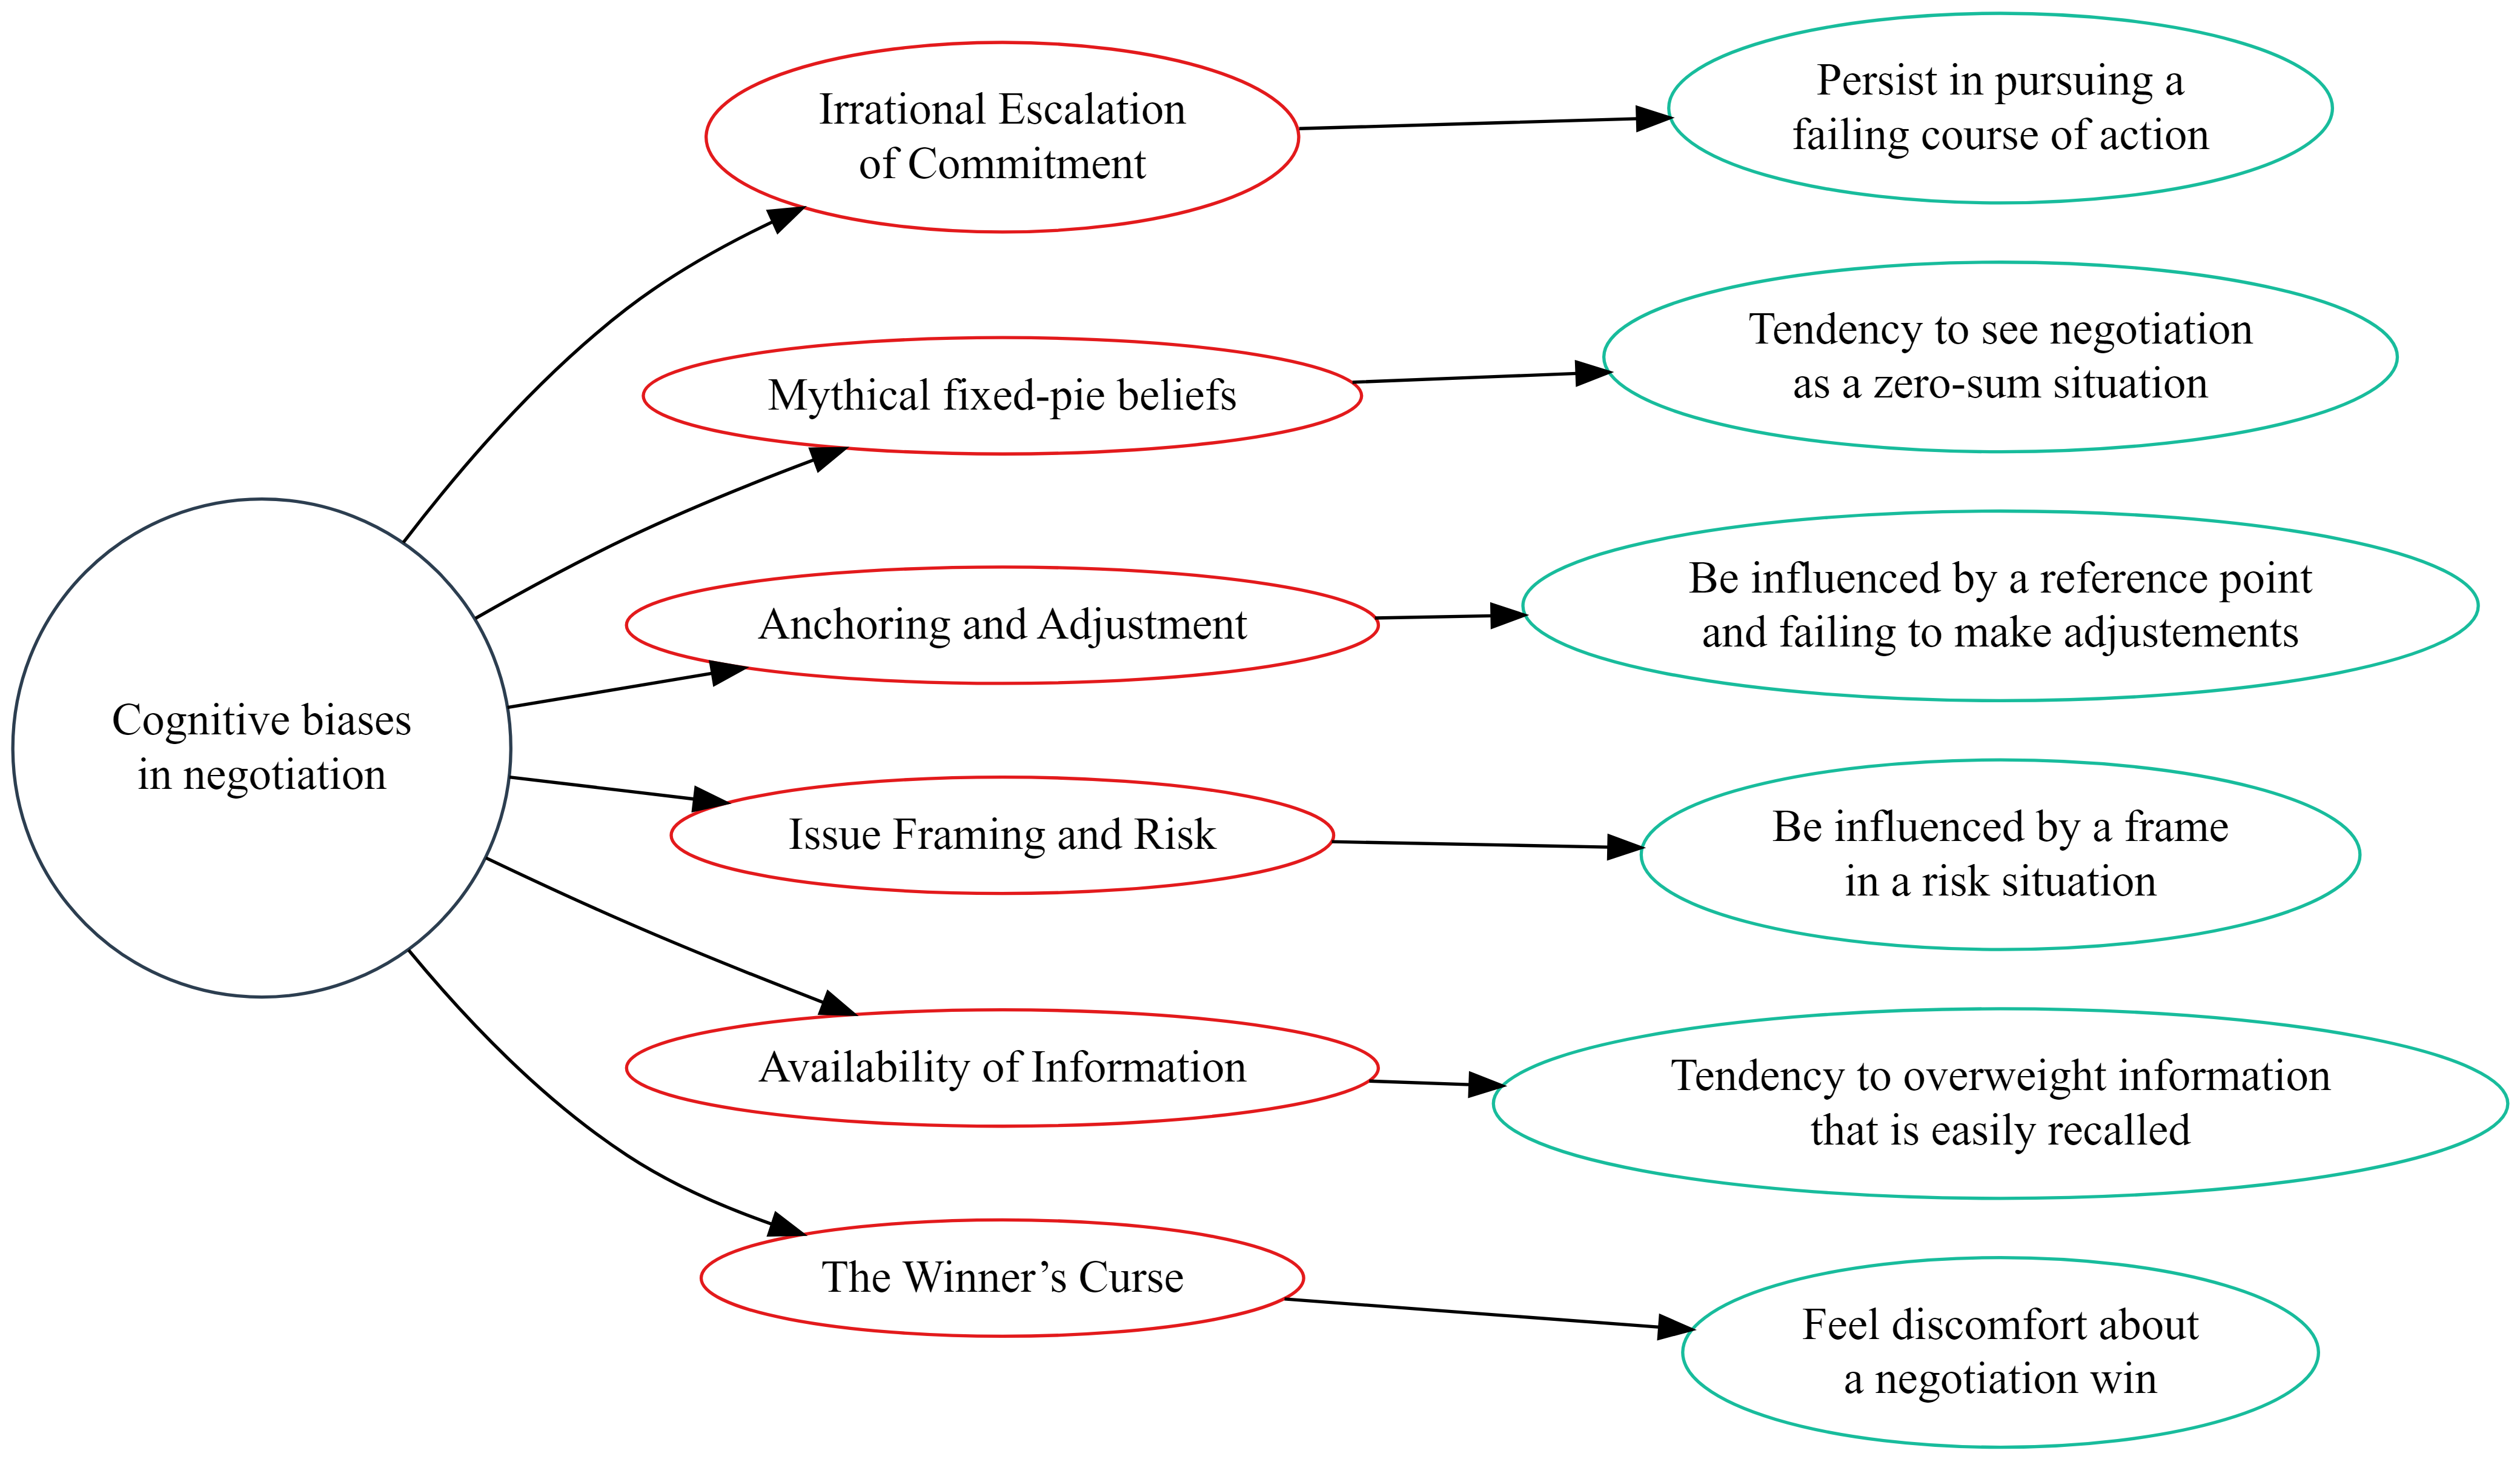
\includegraphics[width=4.5in,height=2.5in]{005_per_cog_emo_files/figure-beamer/dot-figure-1.png}

}

\caption{\label{fig-cognitive-biases-in-negotiation-1}Cognitive biases
in the context of a negotiation\footnote<.->{For a general
  \textbf{cognitive bias} taxonomy check out
  (\citeproc{ref-dimara_task-based_2020}{Dimara et al. 2020})}}

\end{figure}%
\end{frame}

\begin{frame}{}
\phantomsection\label{section-11}
\begin{itemize}
\tightlist
\item
  A \textbf{cognitive bias} is defined as a systematic error that
  affects the decisions and judgments.
\end{itemize}

\begin{figure}

\centering{

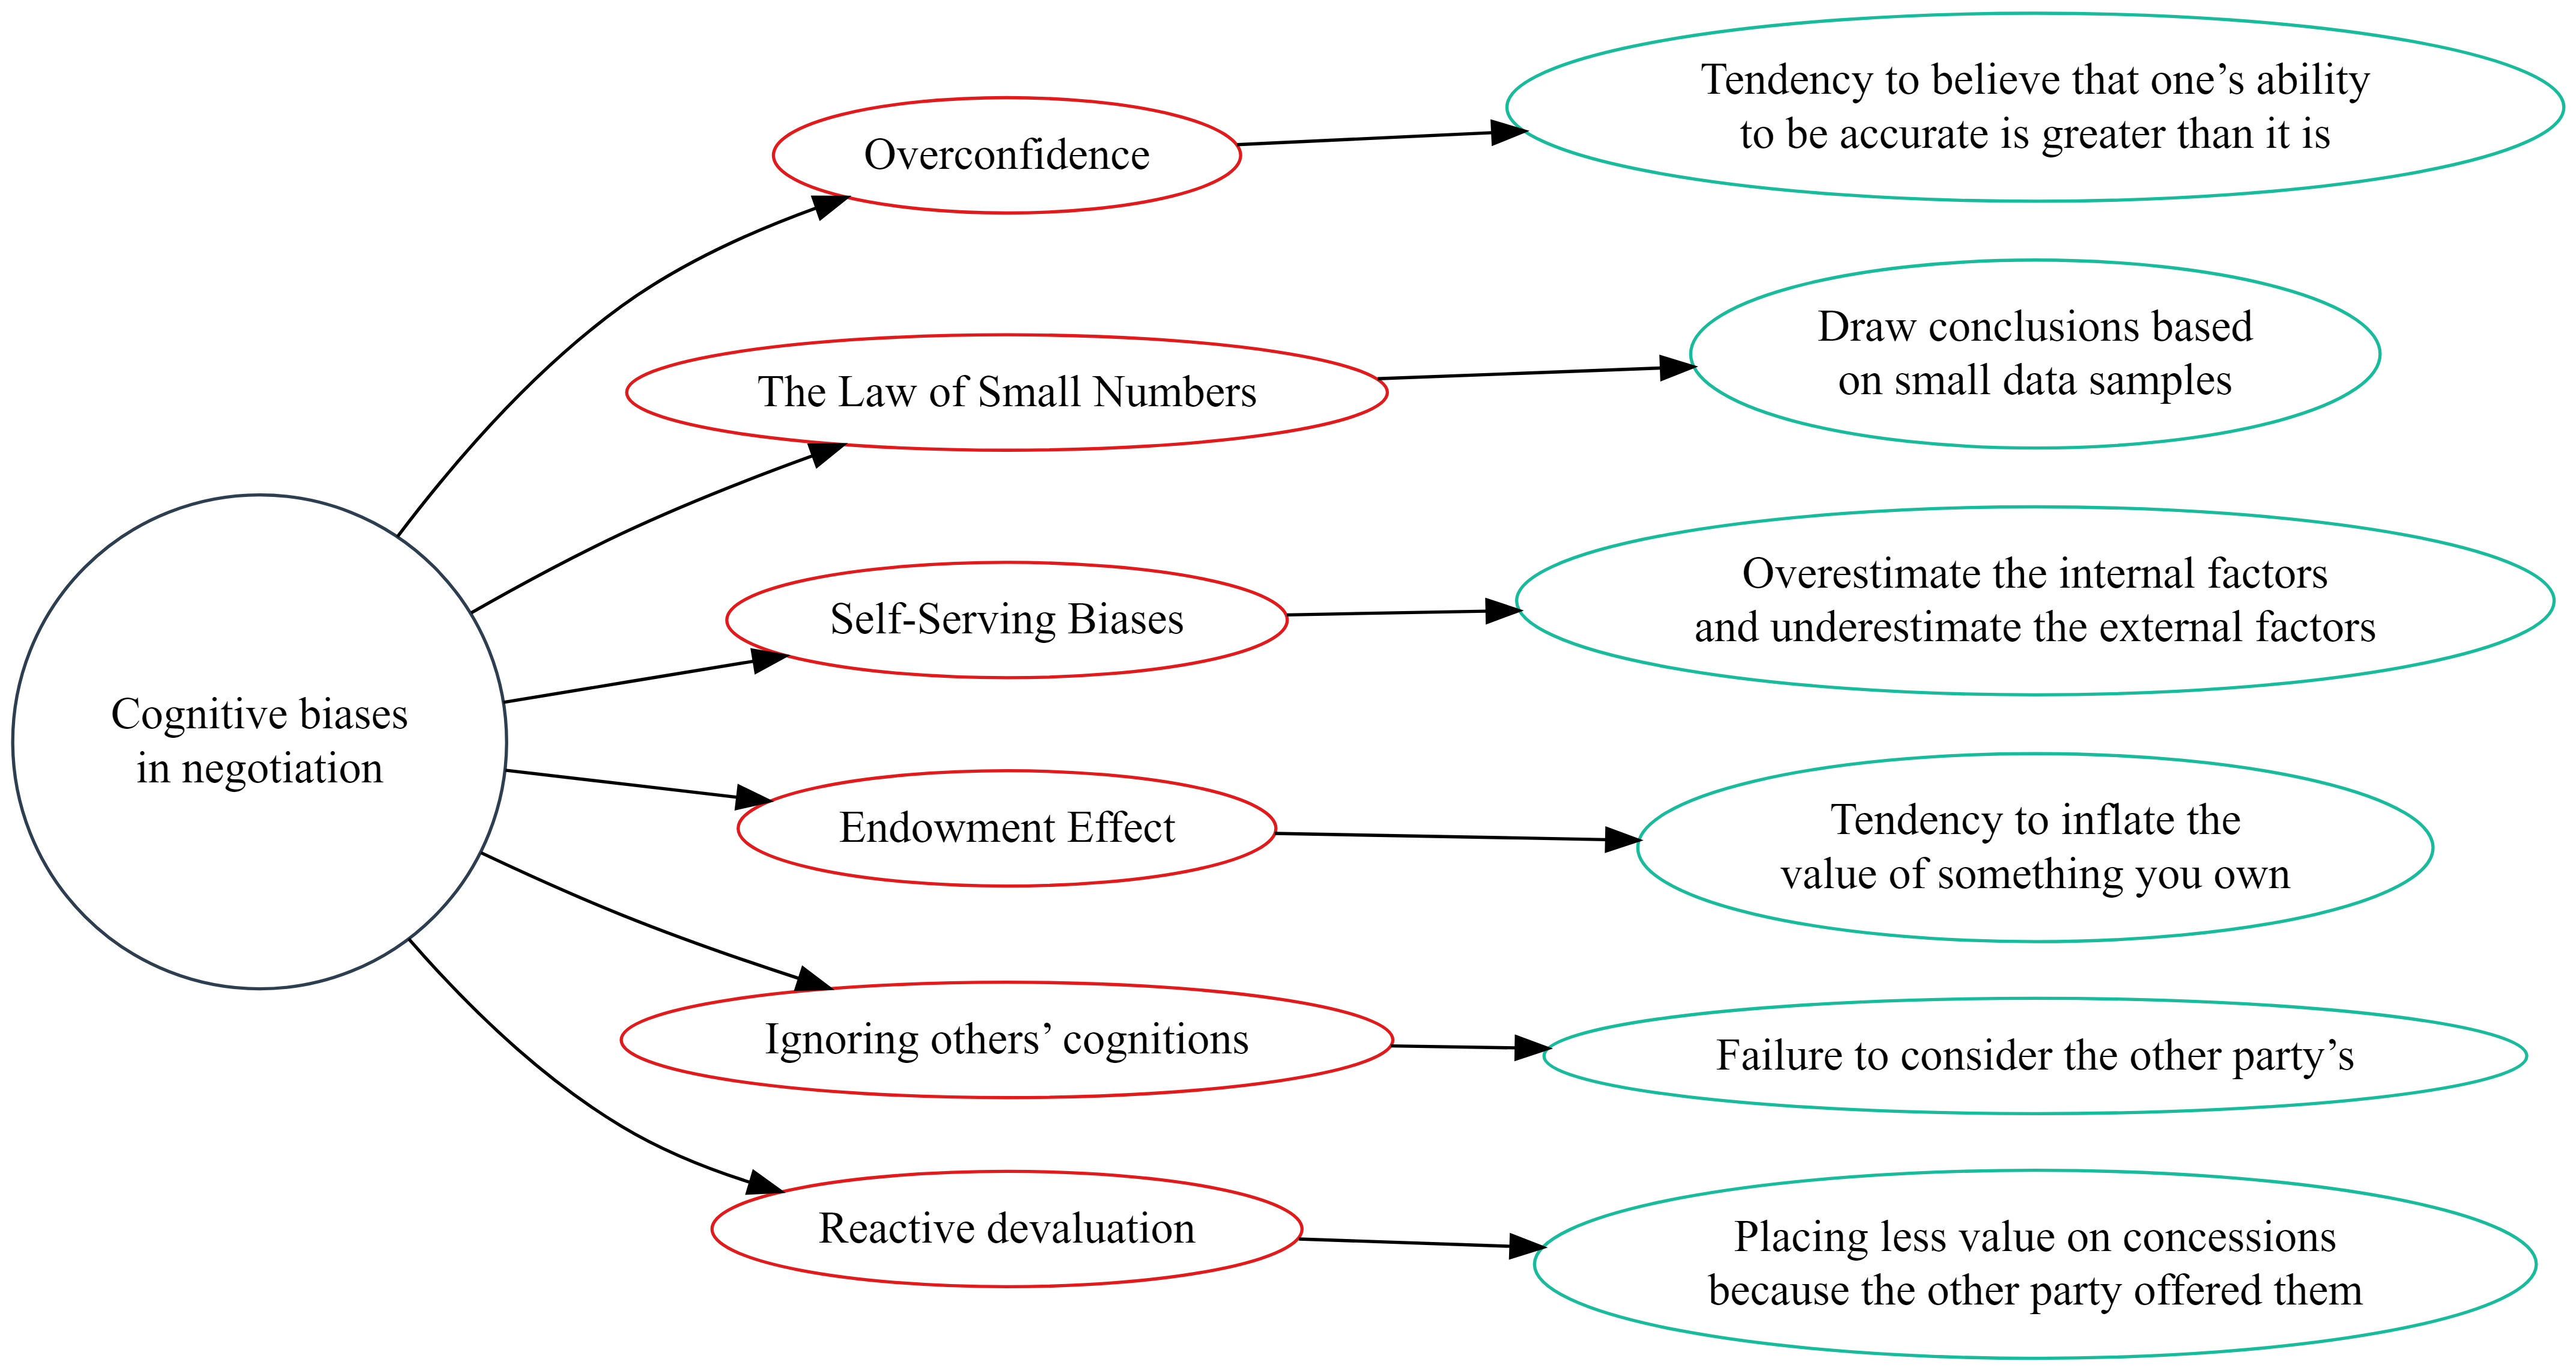
\includegraphics[width=4.5in,height=2.5in]{005_per_cog_emo_files/figure-beamer/dot-figure-6.png}

}

\caption{\label{fig-cognitive-biases-in-negotiation-2}Cognitive biases
in the context of a negotiation\footnote<.->{For a general
  \textbf{cognitive bias} taxonomy check out
  (\citeproc{ref-dimara_task-based_2020}{Dimara et al. 2020})}}

\end{figure}%
\end{frame}

\section{An alternative approach: Mood and
Emotion}\label{an-alternative-approach-mood-and-emotion}

\begin{frame}{}
\phantomsection\label{section-12}
\begin{itemize}
\item
  The study of \textbf{cognitive biases} in negotiation is focused on
  how negotiators make judgment errors or how can negotiators can
  mitigate or eliminate this errors to improve the decision making
  process.
\item
  Another approach is to use emotions as a strategic tool in
  negotiations\footnote<.->{As a conflict negotiation professor I am
    quite bad at using this tool} by adjusting the negotiation stance
  based on the other party's emotional state.
\end{itemize}
\end{frame}

\begin{frame}{}
\phantomsection\label{section-13}
\begin{figure}

\centering{

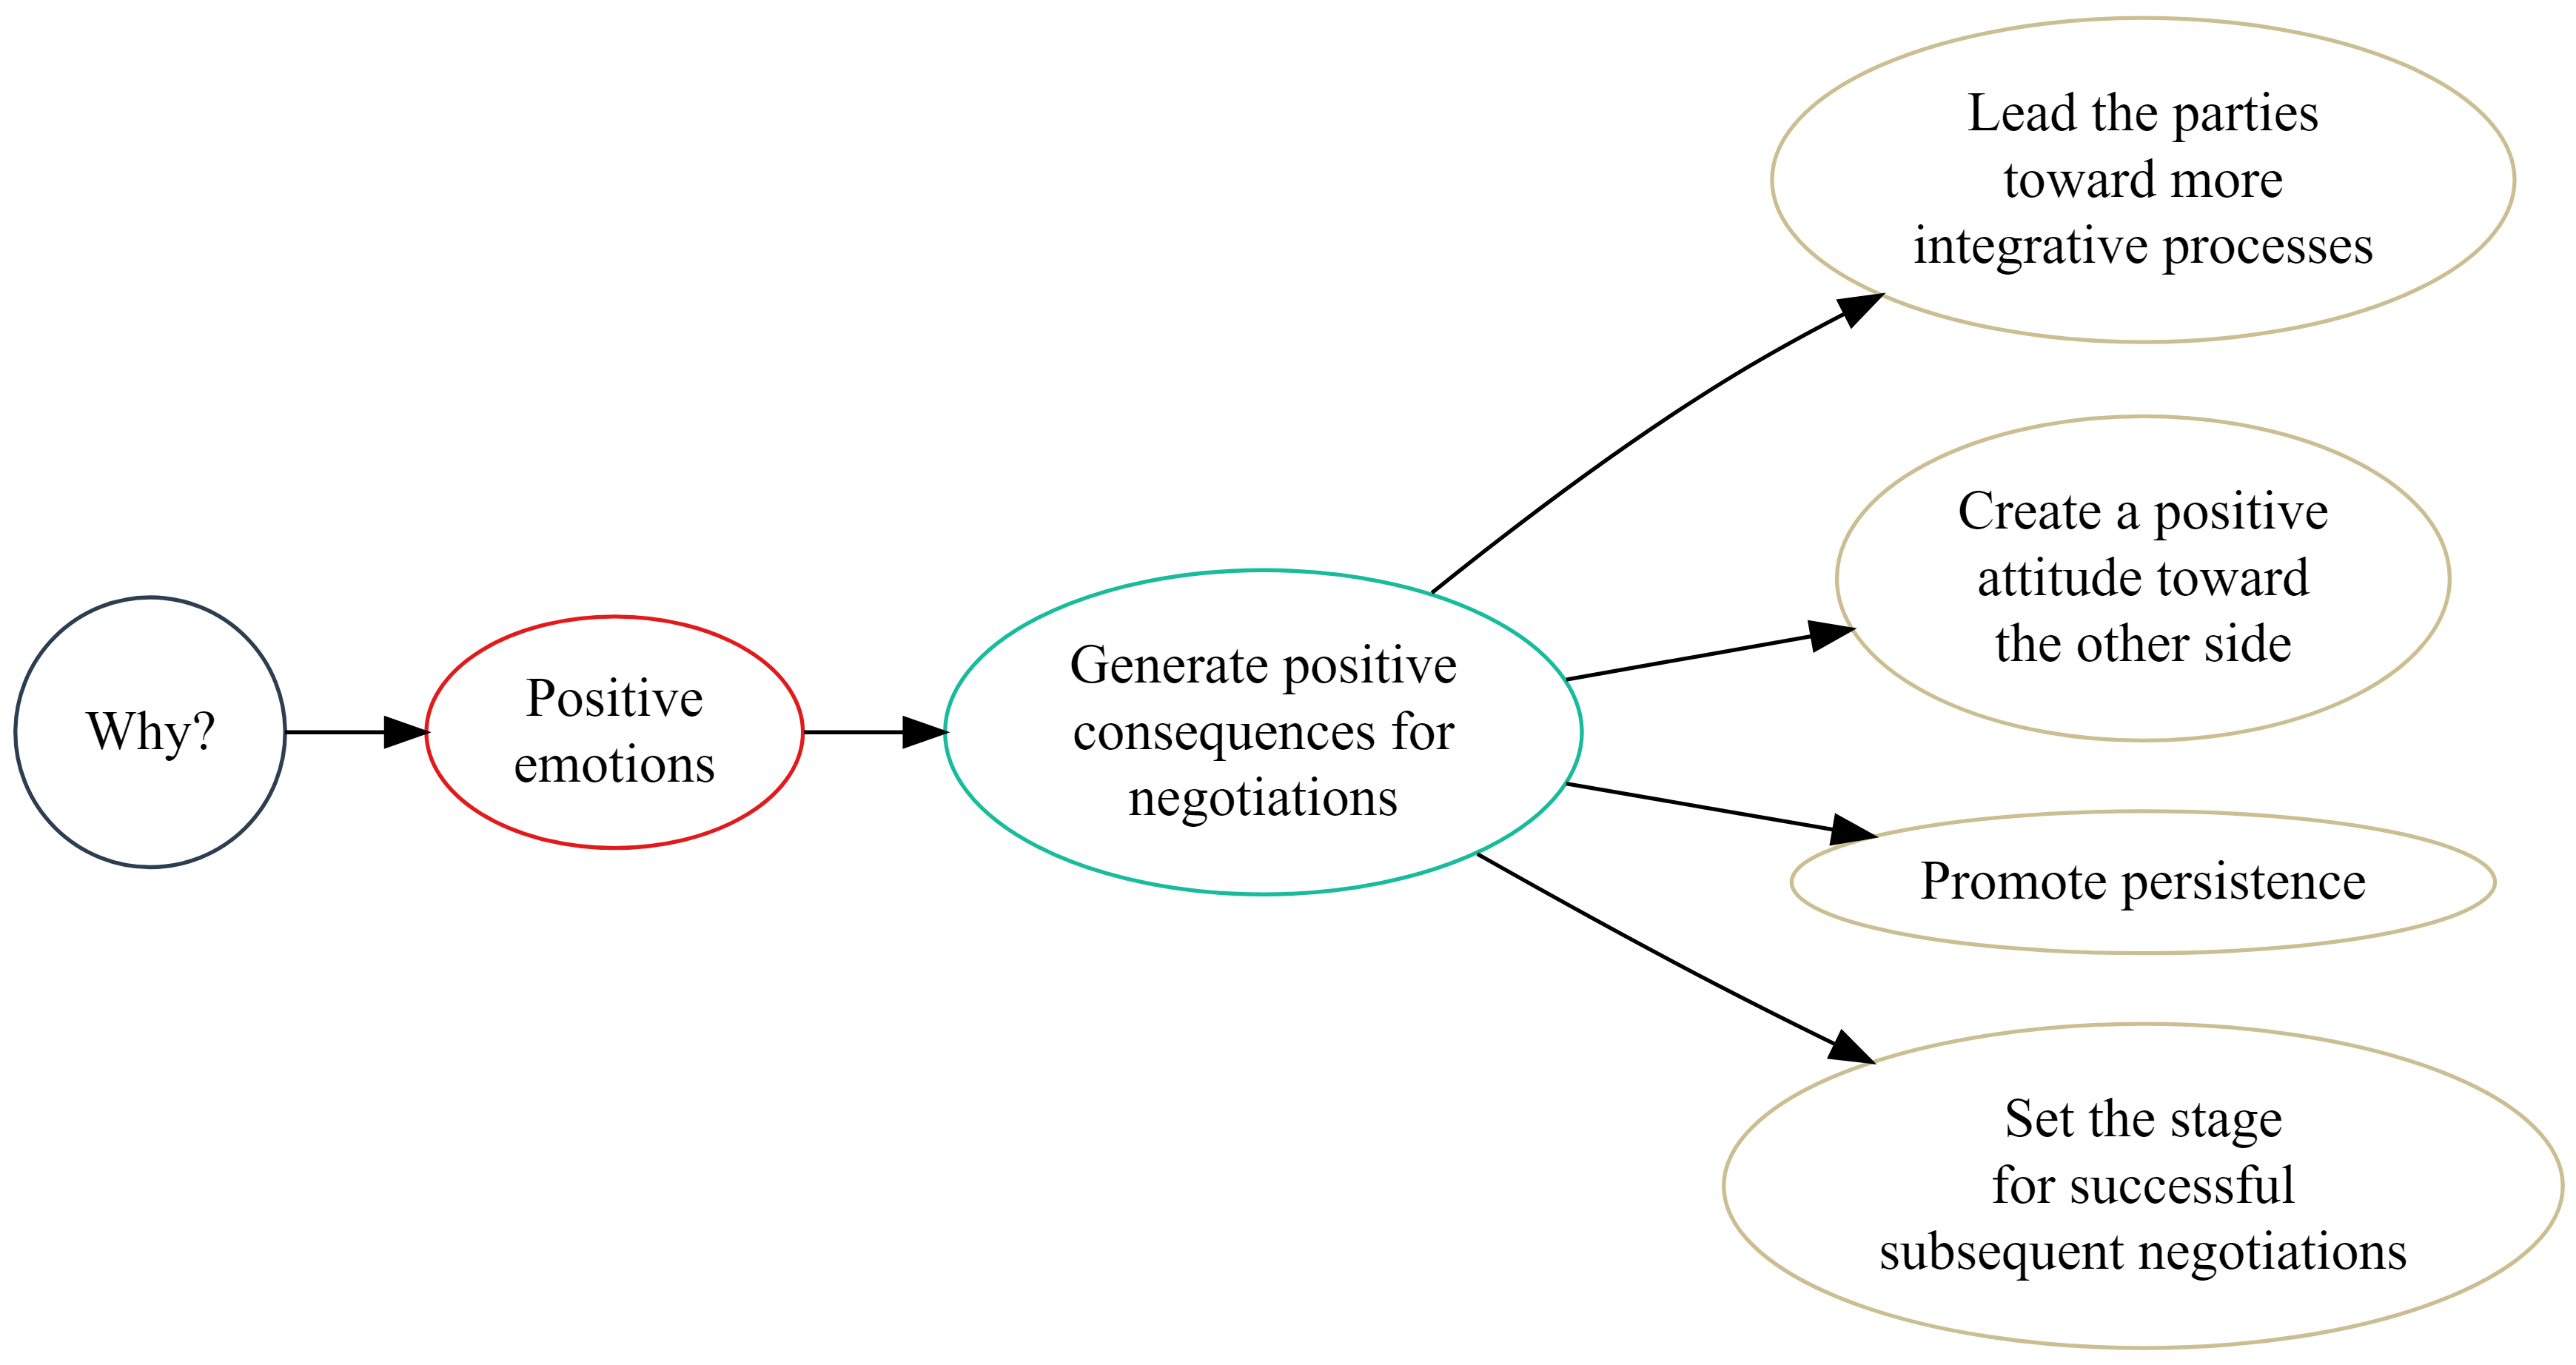
\includegraphics[width=4.5in,height=2.5in]{005_per_cog_emo_files/figure-beamer/dot-figure-5.png}

}

\caption{\label{fig-positive-emotions-consequences}Positive emotions and
consequences for negotiations
(\citeproc{ref-lewicki_negociacion_2024}{Lewicki, Barry, and Saunders
2024}, p 202)}

\end{figure}%
\end{frame}

\begin{frame}{}
\phantomsection\label{section-14}
\begin{figure}

\centering{

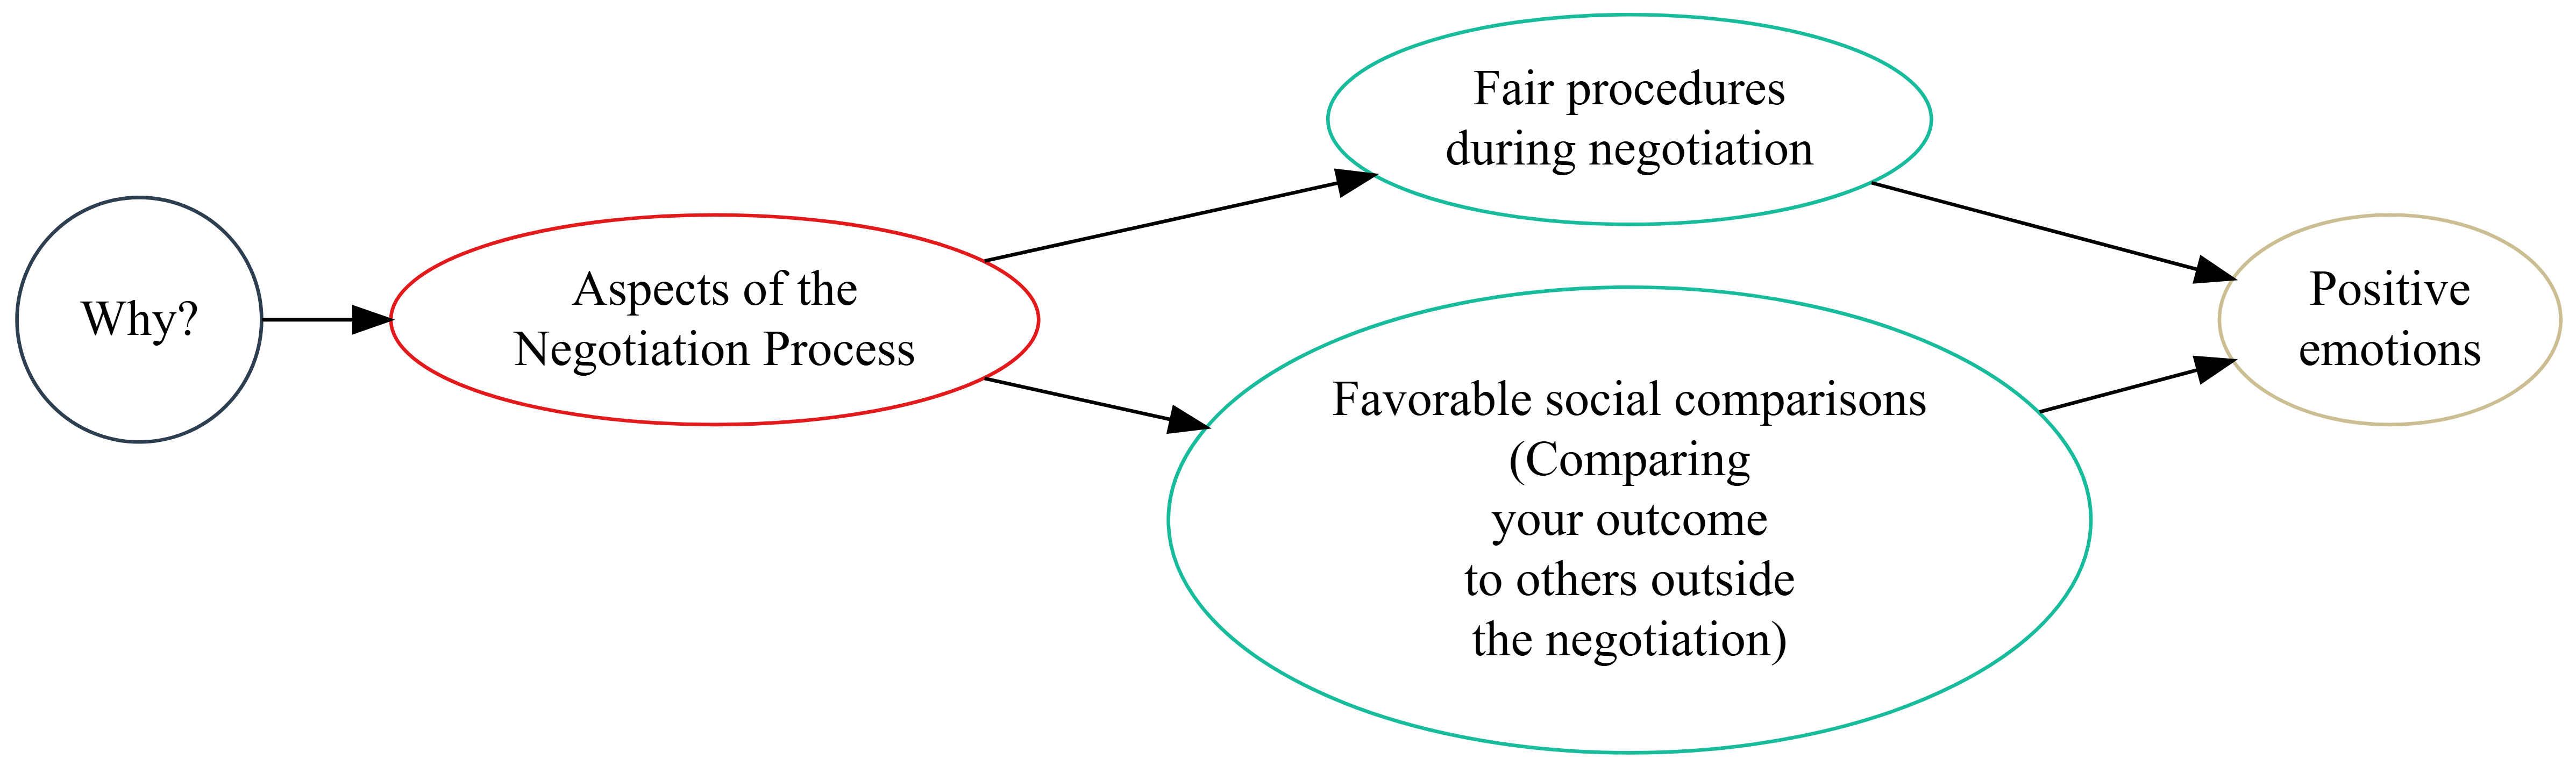
\includegraphics[width=4.5in,height=2.5in]{005_per_cog_emo_files/figure-beamer/dot-figure-4.png}

}

\caption{\label{fig-aspects-negotiation-process-positive-emotions}Aspects
of the negotiation process and positive emotions
(\citeproc{ref-lewicki_negociacion_2024}{Lewicki, Barry, and Saunders
2024}, p 203)}

\end{figure}%
\end{frame}

\begin{frame}{}
\phantomsection\label{section-15}
\begin{figure}

\centering{

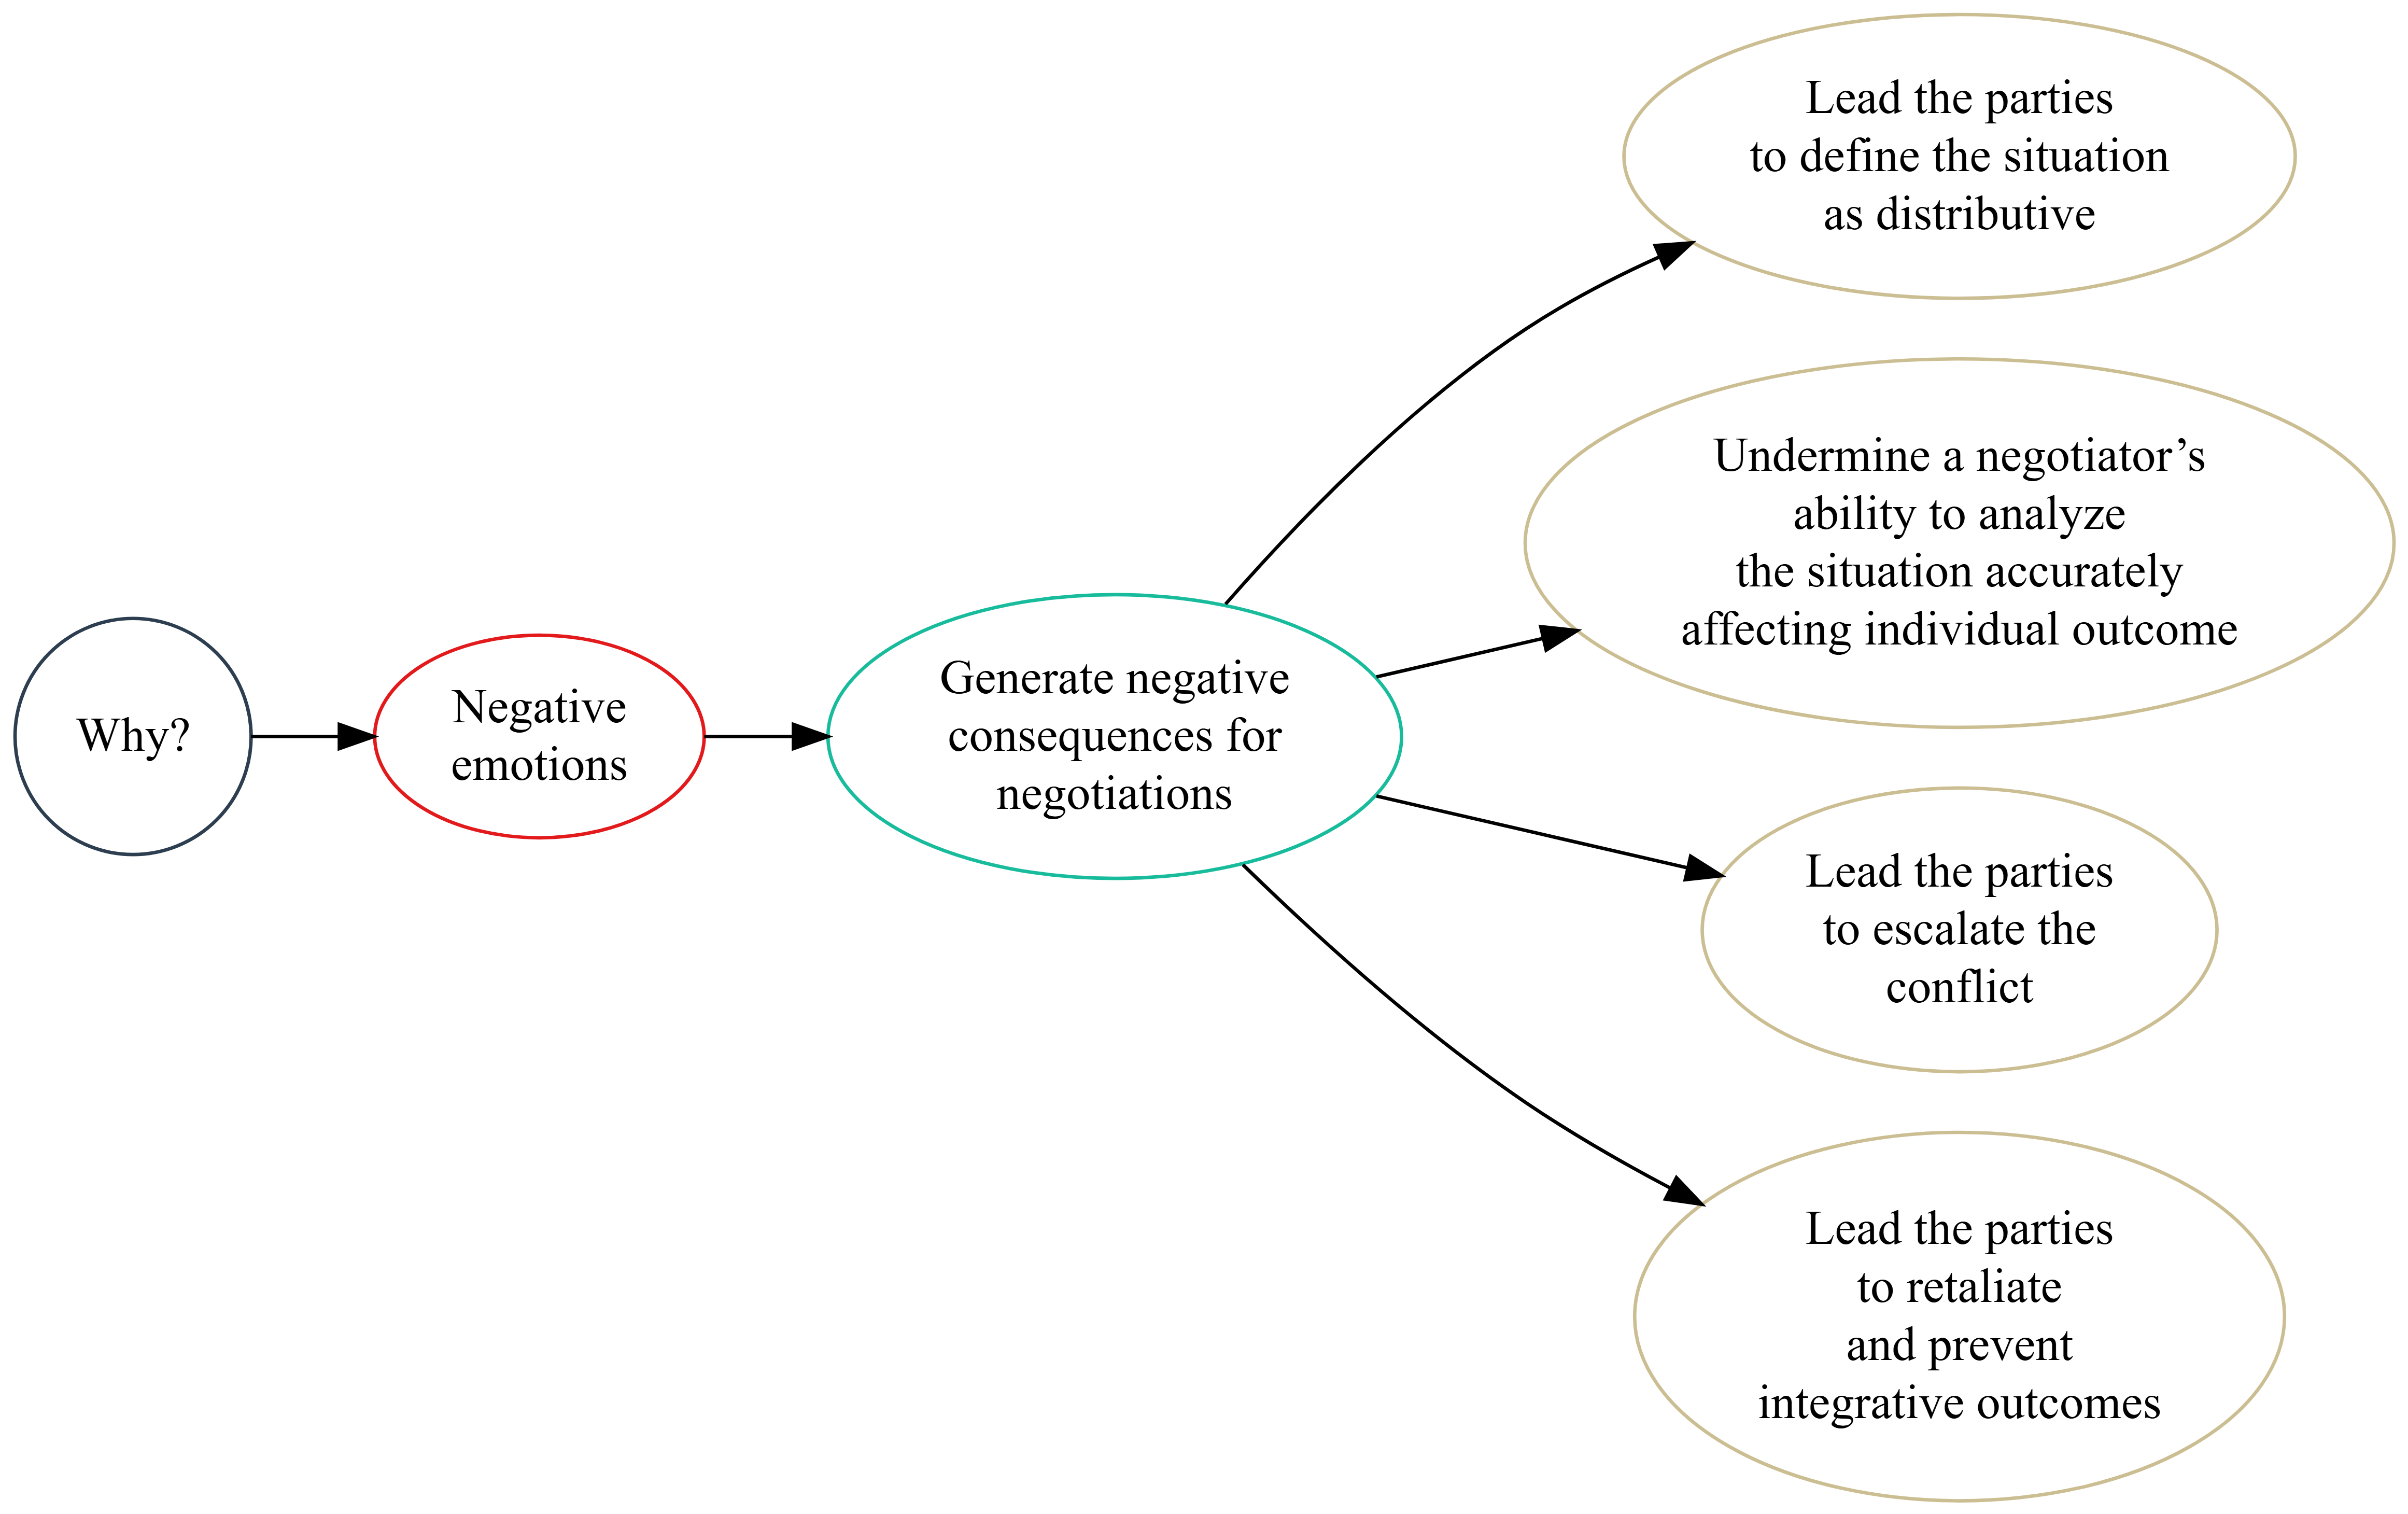
\includegraphics[width=4.5in,height=2.5in]{005_per_cog_emo_files/figure-beamer/dot-figure-3.png}

}

\caption{\label{fig-negative-emotions-consequences}Negative emotions and
consequences for negotiations
(\citeproc{ref-lewicki_negociacion_2024}{Lewicki, Barry, and Saunders
2024}, p 203-204)}

\end{figure}%
\end{frame}

\begin{frame}{}
\phantomsection\label{section-16}
\begin{figure}

\centering{

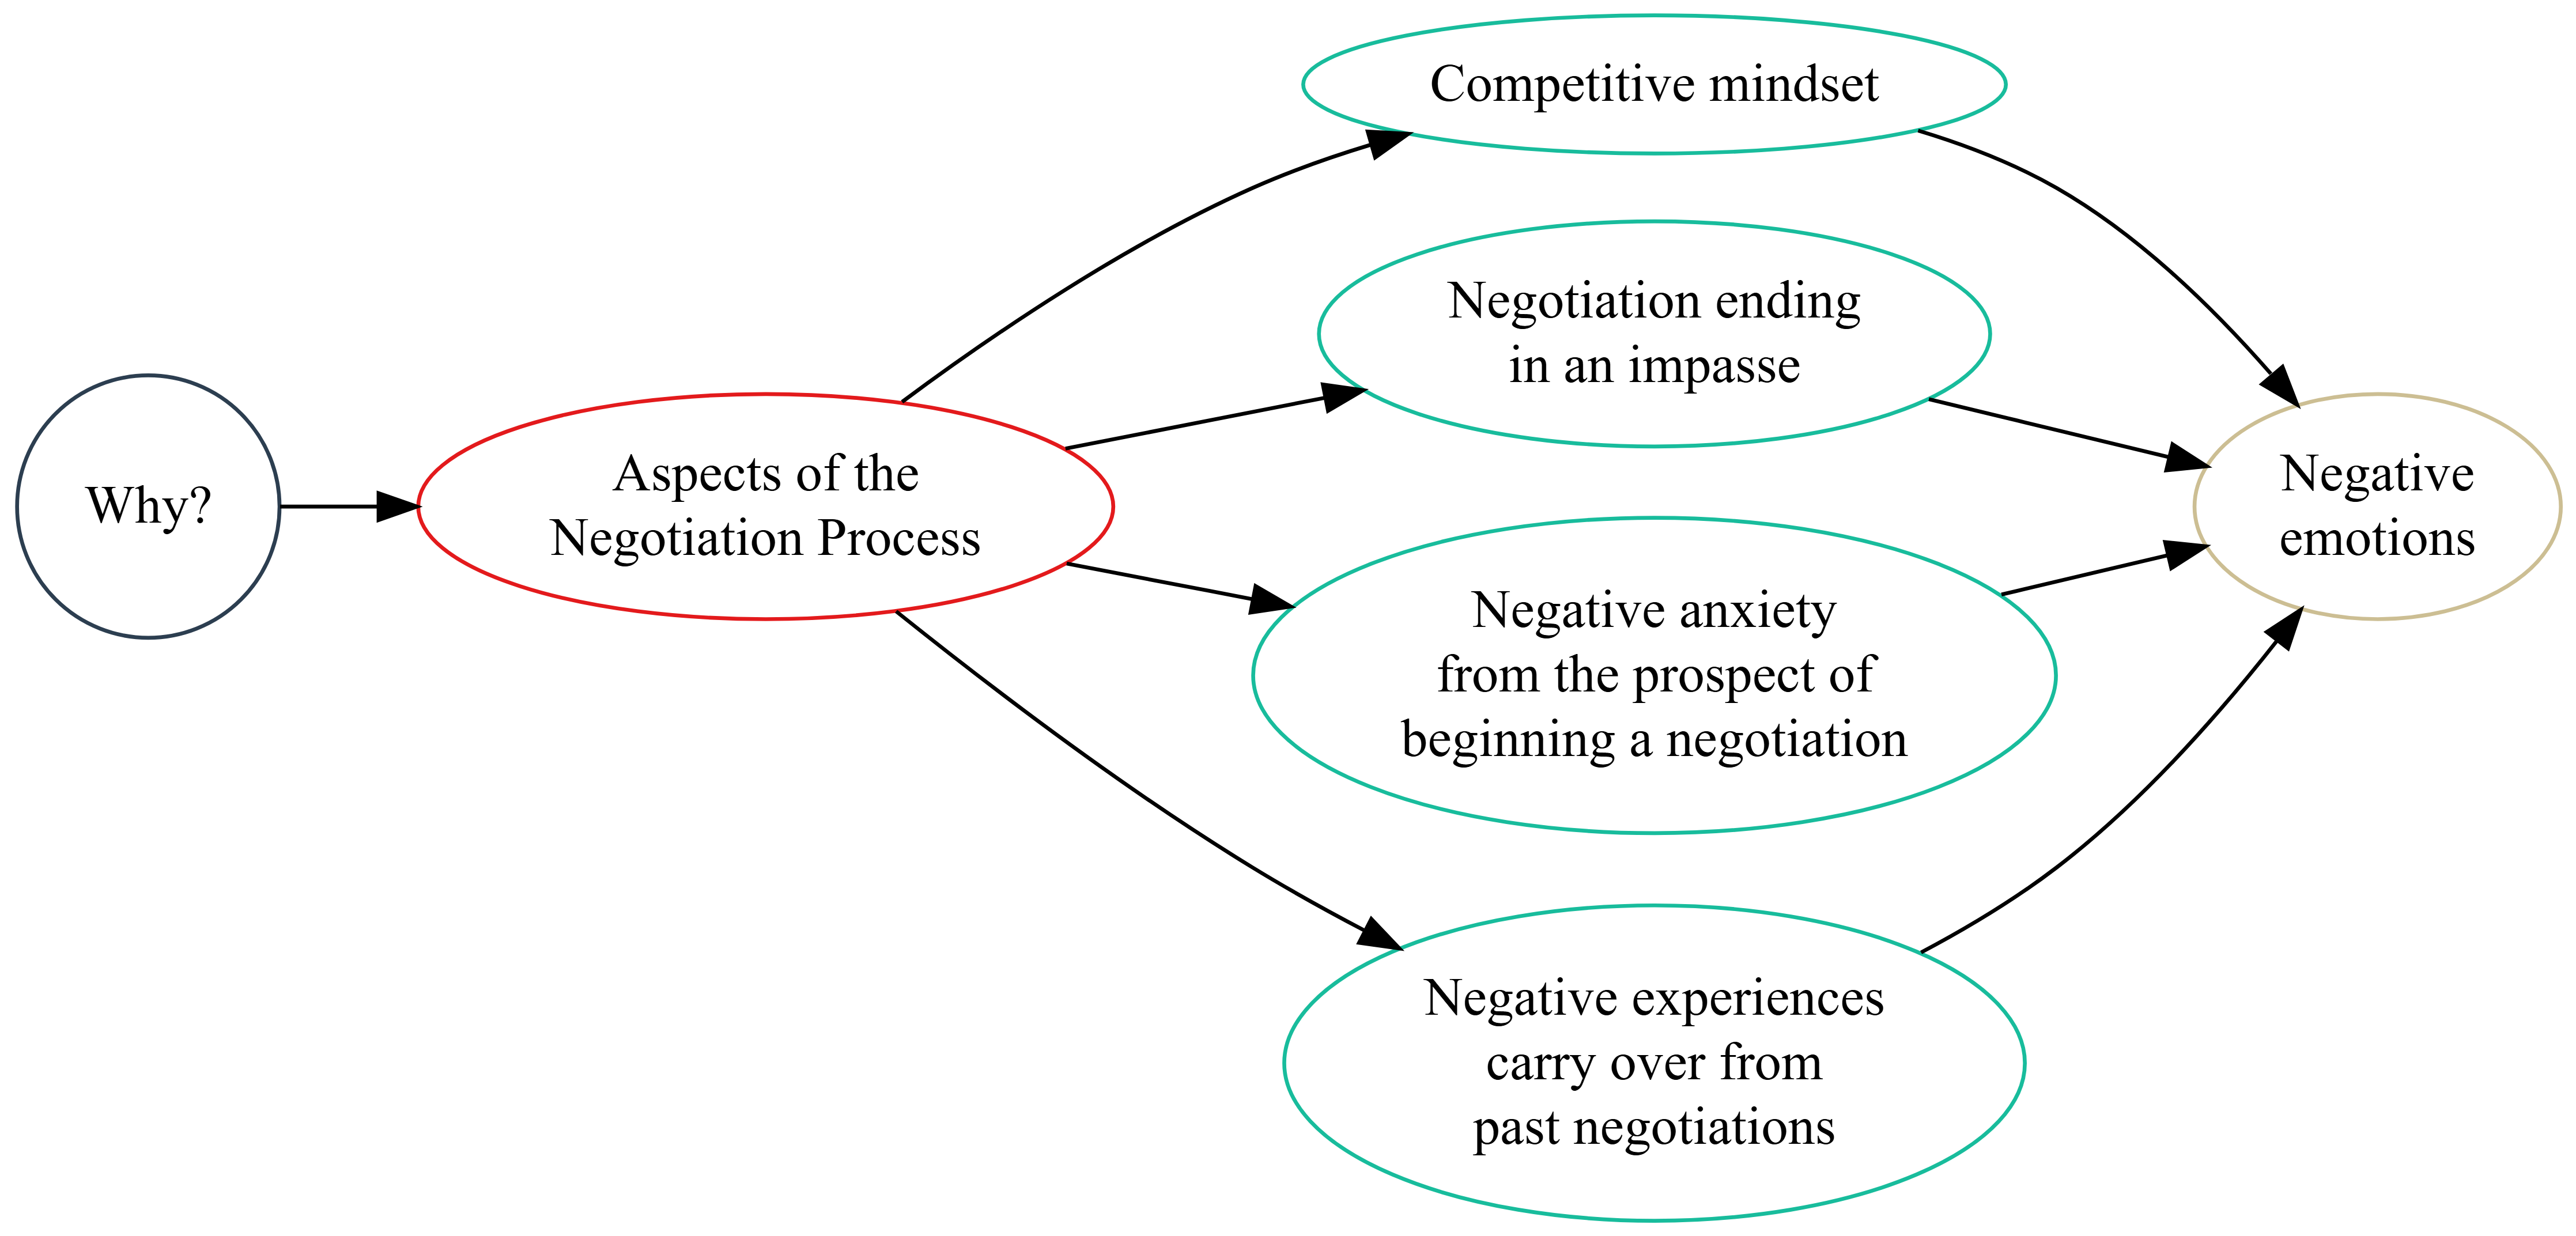
\includegraphics[width=4.5in,height=2.5in]{005_per_cog_emo_files/figure-beamer/dot-figure-2.png}

}

\caption{\label{fig-aspects-negotiation-process-negative-emotions}Aspects
of the negotiation process and negative emotions
(\citeproc{ref-lewicki_negociacion_2024}{Lewicki, Barry, and Saunders
2024}, p 205)}

\end{figure}%
\end{frame}

\section{Acknowledgments}\label{acknowledgments}

\begin{frame}{}
\phantomsection\label{section-17}
\begin{itemize}
\item
  To my family that supports me
\item
  To the taxpayers of Colombia and the
  \href{https://www.umng.edu.co/estudiante}{\textbf{UMNG students}} who
  pay my salary
\item
  To the \href{https://www.business-science.io/}{\textbf{Business
  Science}} and \href{https://www.rfordatasci.com/}{\textbf{R4DS Online
  Learning}} communities where I learn
  \href{https://www.r-project.org/about.html}{\textbf{R}} and
  \href{https://www.python.org/about/}{\textbf{\(\pi\)-thon}}
\item
  To the \href{https://www.r-project.org/contributors.html}{\textbf{R
  Core Team}}, the creators of
  \href{https://rstudio.com/products/rstudio/}{\textbf{RStudio IDE}},
  \href{https://quarto.org/}{\textbf{Quarto}} and the authors and
  maintainers of the packages
  \href{https://CRAN.R-project.org/package=knitr}{\textbf{knitr}}, and
  \href{https://CRAN.R-project.org/package=tinytex}{\textbf{tinytex}}
  for allowing me to access these tools without paying for a license
\item
  To the \href{https://www.kernel.org/category/about.html}{\textbf{Linux
  kernel community}} for allowing me the possibility to use some
  \href{https://static.lwn.net/Distributions/}{\textbf{Linux
  distributions}} as my main
  \href{https://en.wikipedia.org/wiki/Operating_system}{\textbf{OS}}
  without paying for a license
\end{itemize}
\end{frame}

\section*{References}\label{references}
\addcontentsline{toc}{section}{References}

\begin{frame}[allowframebreaks]{References}
\phantomsection\label{refs}
\begin{CSLReferences}{1}{0}
\bibitem[\citeproctext]{ref-adelson_checkershadow_1995}
Adelson, Edward H. 1995. {``Checkershadow {Illusion}.''}
\url{http://persci.mit.edu/gallery/checkershadow}.

\bibitem[\citeproctext]{ref-bateson_steps_2000}
Bateson, Gregory. 2000. \emph{Steps to an Ecology of Mind}. University
of Chicago Press ed. Chicago: University of Chicago Press.

\bibitem[\citeproctext]{ref-dimara_task-based_2020}
Dimara, Evanthia, Steven Franconeri, Catherine Plaisant, Anastasia
Bezerianos, and Pierre Dragicevic. 2020. {``A {Task}-{Based} {Taxonomy}
of {Cognitive} {Biases} for {Information} {Visualization}.''} \emph{IEEE
Transactions on Visualization and Computer Graphics} 26 (2): 1413--32.
\url{https://doi.org/10.1109/TVCG.2018.2872577}.

\bibitem[\citeproctext]{ref-goffman_frame_1986}
Goffman, Erving. 1986. \emph{Frame Analysis: An Essay on the
Organization of Experience}. Northeastern University Press ed. Boston:
Northeastern University Press.

\bibitem[\citeproctext]{ref-iyengar_when_2000}
Iyengar, Sheena S., and Mark R. Lepper. 2000. {``When Choice Is
Demotivating: {Can} One Desire Too Much of a Good Thing?''}
\emph{Journal of Personality and Social Psychology} 79 (6): 995--1006.
\url{https://doi.org/10.1037/0022-3514.79.6.995}.

\bibitem[\citeproctext]{ref-leonardelli_multiple_2019}
Leonardelli, Geoffrey J., Jun Gu, Geordie McRuer, Victoria Husted
Medvec, and Adam D. Galinsky. 2019. {``Multiple Equivalent Simultaneous
Offers ({MESOs}) Reduce the Negotiator Dilemma: {How} a Choice of First
Offers Increases Economic and Relational Outcomes.''}
\emph{Organizational Behavior and Human Decision Processes} 152 (May):
64--83. \url{https://doi.org/10.1016/j.obhdp.2019.01.007}.

\bibitem[\citeproctext]{ref-lewicki_negociacion_2024}
Lewicki, Roy J., Bruce Barry, and David M. Saunders. 2024.
\emph{Negociación}. 9th ed. McGraw-Hill Education.
\url{https://www-ebooks7-24-com.ezproxy.umng.edu.co/?il=40562}.

\bibitem[\citeproctext]{ref-luckiesh_visual_2017}
Luckiesh, Matthew. 2017. \emph{Visual Illusions: Their Causes,
Characteristics and Applications}.

\bibitem[\citeproctext]{ref-shonk_framing_2020}
Shonk, Katie. 2020. {``Framing in {Negotiation}.''} \emph{PON - Program
on Negotiation at Harvard Law School}.
\url{https://www.pon.harvard.edu/daily/business-negotiations/framing-in-negotiation/}.

\bibitem[\citeproctext]{ref-simonson_choice_1992}
Simonson, Itamar, and Amos Tversky. 1992. {``Choice in {Context}:
{Tradeoff} {Contrast} and {Extremeness} {Aversion}.''} \emph{Journal of
Marketing Research} 29 (3): 281. \url{https://doi.org/10.2307/3172740}.

\bibitem[\citeproctext]{ref-tversky_framing_1981}
Tversky, A, and D Kahneman. 1981. {``The Framing of Decisions and the
Psychology of Choice.''} \emph{Science} 211 (4481): 453--58.
\url{https://doi.org/10.1126/science.7455683}.

\bibitem[\citeproctext]{ref-zeman_muller-lyer_2013}
Zeman, Astrid, Oliver Obst, Kevin R. Brooks, and Anina N. Rich. 2013.
{``The {Müller}-{Lyer} {Illusion} in a {Computational} {Model} of
{Biological} {Object} {Recognition}.''} Edited by Kevin Paterson.
\emph{PLoS ONE} 8 (2): e56126.
\url{https://doi.org/10.1371/journal.pone.0056126}.

\end{CSLReferences}
\end{frame}




\end{document}
